% Provenance (never printed): see sources/outline_sources.md (Year 2: the vanished ocean;
% ophiolites; nappes; high-pressure rocks; foreland basins; reconstructing the history from
% maps, sections and geophysics). Units, ages and architecture after Schmid et al. (2004);
% Monte Cervino sheet notes (ISPRA 2016); Penrose definition as quoted by Coleman (1984);
% Zermatt-Saas ages Rubatto et al. (1998), Halama et al. (2020); Chenaillet Corno et al.
% (2023); Moho picks Michailos et al. (2023, Zenodo, CC BY 4.0); gravity Zahorec et al.
% (2021); Jura Lanza et al. (2022), Schori et al. (2015); shortening Rosenberg et al.
% (2021); Glarus thrust Herwegh et al. (2008); Molasse Krenmayr (1999), Garefalakis and
% Schlunegger (2018), Sinclair (1997); present uplift Champagnac et al. (2009). Figure data
% in figdata/bachelor-2/alps.py; exercise and problem values in the Book 4 scratch
% calculator calc/ch13.py.
\chapter{Anatomía de una cordillera: los Alpes}\label{ch:b2:alpine-orogen}

La cima del Cervino está hecha de gneis y gabro que pertenecieron en su día al margen
de Apulia, el continente que se extendía del lado de África de un océano desaparecido. Las laderas de debajo
son el fondo de ese océano, serpentinita, gabro y basalto en almohadilla convertidos en eclogita, y
más abajo, en el vecino Monte Rosa, está el borde de Europa. Al ascender por el
apilamiento se pasa de un continente, a través de un océano, al otro. Este capítulo lee los Alpes como un apilamiento así: de dónde vinieron sus piezas, cómo se
apilaron, cuánto terreno se tragó el apilamiento y qué ve la geofísica debajo.
% ledger: ispra16:cervino, schmid04:apulia, schmid04:alpine-tethys

\begin{recall}
\textbf{Del volumen de bachillerato}: la colisión continental, la sutura, el acortamiento de una
capa (la fracción de su longitud que pierde), las fallas inversas y los cabalgamientos. \textbf{Del volumen de primer
año}: los mapas y cortes geológicos; las fallas normales, inversas y de cabalgamiento, los pliegues y
la vergencia; los márgenes pasivos; la corteza oceánica, la lava en almohadilla y el complejo de \omterm{def:b2:magma-emplacement:bodies}{diques}
laminados; los márgenes activos y el prisma de acreción; la isostasia, la raíz de Airy y la anomalía de Bouguer;
la \omterm{def:b2:alpine-orogen:foreland}{cuenca de antepaís} citada entre las cuencas sedimentarias. \textbf{Del
\cref{ch:b2:metamorphic-facies}}: las facies de esquistos azules y de eclogitas. \textbf{Del
\cref{ch:b2:pt-paths}}: las \omterm{def:b2:pt-paths:ptt}{trayectorias P--T--t}, las \omterm{def:b2:pt-paths:exhumation}{tasas de exhumación} y el \omterm{def:b2:pt-paths:uhp}{metamorfismo de ultra alta
presión}.
\end{recall}

\begin{definition}[Orógeno]\label{def:b2:alpine-orogen:orogen}
Un \emph{orógeno}\index{orógeno} es una franja de la litosfera acortada y engrosada por la
convergencia de dos placas, junto con las rocas deformadas y metamorfizadas en ella; la
cordillera es su expresión en superficie, y la corteza engrosada de debajo, su raíz.
\end{definition}

\section{Un océano desaparecido}\label{sec:b2:alpine-orogen:tethys}

Los Alpes registran el cierre de océanos mientras convergían las placas africana y europea.
El principal es el \emph{Tetis alpino}, formado por dos ramas. Su rama meridional, el
océano Piamonte--Liguria, empezó a abrirse en el Jurásico Medio, a la vez que se abría el Atlántico
Central: el Tetis alpino pertenece cinemáticamente a la apertura del Atlántico, a diferencia de los
océanos tetisianos situados más al este. Las radiolaritas, fangos silíceos del mar profundo convertidos en roca,
y las calizas de aptychus siguieron al comienzo de la expansión, y todavía identifican sus
restos. Una estrecha rama septentrional, el océano Valais, se abrió probablemente en el Cretácico
más temprano. Entre ambas se extendía una franja de continente, la cinta brianzonesa, que se adelgaza
hacia el este y falta en los Alpes orientales.
% ledger: schmid04:alpine-tethys

Al norte el océano estaba bordeado por el margen pasivo de Europa, tema del capítulo de los rifts y
los márgenes del volumen de primer año. Al sur se extendía \emph{Apulia}: todo el terreno continental
al sur del Tetis alpino y al norte del Neotetis, más joven, incluido el antepaís
que hoy queda al sur de los Alpes. La cima del Cervino es un fragmento de ella.
% ledger: schmid04:apulia
El mapa siguiente sitúa la cordillera y los lugares de este capítulo.

\begin{omfigure}
\centering
% ledger: data:b4-etopo-alps, schmid04:windows, schmid04:foreland, ispra16:cervino
\begin{tikzpicture}
\begin{axis}[width=0.96\linewidth, height=0.74\linewidth, xmin=5, xmax=14, ymin=43.5,
  ymax=48.5, xlabel={longitud (\unit{\degree} E)}, ylabel={latitud (\unit{\degree} N)},
  tick label style={font=\scriptsize}, label style={font=\small}, clip=true,
  xtick={5,6,...,14}, ytick={44,45,...,48}]
\addplot[omThm!35, line width=0.3pt] table[x=lon, y=lat] {figdata/out/bachelor-2-alps-c1000.dat};
\addplot[omThm!90!black, line width=0.45pt] table[x=lon, y=lat] {figdata/out/bachelor-2-alps-c2000.dat};
\addplot[blue!60!black, line width=0.5pt] table[x=lon, y=lat] {figdata/out/bachelor-2-alps-c0.dat};
\draw[red!70!black, line width=1pt] (axis cs:8,45.3) -- (axis cs:8,48.0);
\node[font=\scriptsize\bfseries, red!70!black, anchor=north west] at (axis cs:8.02,45.32) {A};
\node[font=\scriptsize\bfseries, red!70!black, anchor=south west] at (axis cs:8.02,47.98) {B};
\fill (axis cs:6.865,45.833) circle (1.3pt) node[font=\scriptsize, fill=white, fill opacity=0.85, text opacity=1, inner sep=1pt, anchor=north east] {Mont Blanc};
\fill (axis cs:7.659,45.976) circle (1.3pt) node[font=\scriptsize, fill=white, fill opacity=0.85, text opacity=1, inner sep=1pt, anchor=south east] {Cervino};
\node[font=\scriptsize\itshape, rotate=40] at (axis cs:6.35,46.85) {Jura};
\node[font=\scriptsize\itshape] at (axis cs:9.35,47.65) {cuenca de la Molasa};
\node[font=\scriptsize\itshape] at (axis cs:10.0,45.05) {llanura del Po};
\node[font=\scriptsize\itshape, align=center, fill=white, fill opacity=0.8, text opacity=1, inner sep=1pt] at (axis cs:10.3,46.95) {ventana de\\la Engadina};
\node[font=\scriptsize\itshape, align=center, fill=white, fill opacity=0.8, text opacity=1, inner sep=1pt] at (axis cs:12.6,47.25) {ventana de\\los Tauern};
\node[font=\scriptsize\itshape] at (axis cs:8.6,43.85) {mar de Liguria};
\end{axis}
\end{tikzpicture}
\par\smallskip{\small Los Alpes según el modelo de relieve ETOPO1, con nodos separados
\qty{0.05}{\degree}: curvas de nivel de \qty{1000}{m} (claras) y \qty{2000}{m} (oscuras) y la línea de costa. El
nodo más alto de esta malla está a \qty{3914}{m}, cerca del Mont Blanc; las cumbres son más altas,
porque un nodo de la malla muestrea una celda, no una cima. La línea A--B a lo largo de \qty{8}{\degree} E es
el perfil dibujado en la última sección del capítulo. Nombres de los accidentes colocados a mano en sus
posiciones aproximadas.}
\end{omfigure}

¿Cómo se puede conocer un océano que ya no existe? Por fragmentos de su fondo que escaparon a la
subducción y quedaron atrapados en la cordillera.

\begin{definition}[Ofiolita; secuencia ofiolítica de Penrose]\label{def:b2:alpine-orogen:ophiolite}
Una \emph{ofiolita}\index{ofiolita} es una asociación característica de rocas máficas a
ultramáficas, un fragmento de litosfera oceánica que hoy se encuentra en tierra firme. La \emph{secuencia ofiolítica
de Penrose}\index{secuencia ofiolítica de Penrose} es la asociación completa definida por una
conferencia de geólogos en 1972; de abajo arriba:
\begin{enumerate}
\item un complejo ultramáfico de \omterm{def:b2:mantle-melting:peridotites}{harzburgita}, \omterm{def:b2:mantle-melting:peridotites}{lherzolita} y \omterm{def:b2:mantle-melting:peridotites}{dunita}, normalmente con una
fábrica de deformación adquirida en estado sólido;
\item un complejo gabroico, de ordinario con texturas de \omterm{def:b2:magmatic-differentiation:cumulate}{cumulado};
\item un complejo máfico de \omterm{def:b2:magma-emplacement:bodies}{diques} laminados;
\item un complejo volcánico máfico, a menudo en almohadillas.
\end{enumerate}
\end{definition}
% ledger: coleman84:penrose

La definición de Penrose fue un consenso, criticado desde el principio, y todavía aceptado en general.
Su secuencia es la estratificación de la corteza oceánica y del manto superior vista en el volumen de primer
año: lavas en almohadilla sobre \omterm{def:b2:magma-emplacement:bodies}{diques} laminados, sobre gabro, sobre el manto. Las \omterm{def:b2:alpine-orogen:ophiolite}{ofiolitas}, sin embargo, no son
un fondo oceánico medio. La mayor parte de la corteza abisal, la de los océanos amplios, se consume por
subducción; Coleman sostuvo que las \omterm{def:b2:alpine-orogen:ophiolite}{ofiolitas} de los cinturones alpino y cordillerano se formaron
sobre todo en los centros de expansión de pequeñas cuencas oceánicas o entre arcos insulares, y que las
tetisianas se formaron donde la corteza continental se adelgazó a lo largo de márgenes pasivos hasta que se abrió un pequeño
océano.
% ledger: coleman84:penrose, coleman84:settings

Las \omterm{def:b2:alpine-orogen:ophiolite}{ofiolitas} alpinas encajan en ese cuadro. Las unidades procedentes del océano Piamonte--Liguria
son restos de litosfera oceánica y de manto que había subido desde debajo del
continente adelgazado, el manto subcontinental, y había quedado expuesto en el fondo marino. En el
Chenaillet, en los Alpes occidentales, la mejor conservada de ellas muestra manto
expuesto, gabros y una famosa secuencia de basaltos en almohadilla, sin cobertera sedimentaria.
La fotografía siguiente los muestra.
% ledger: schmid04:units, corno23:chenaillet

\begin{omfigure}
\centering
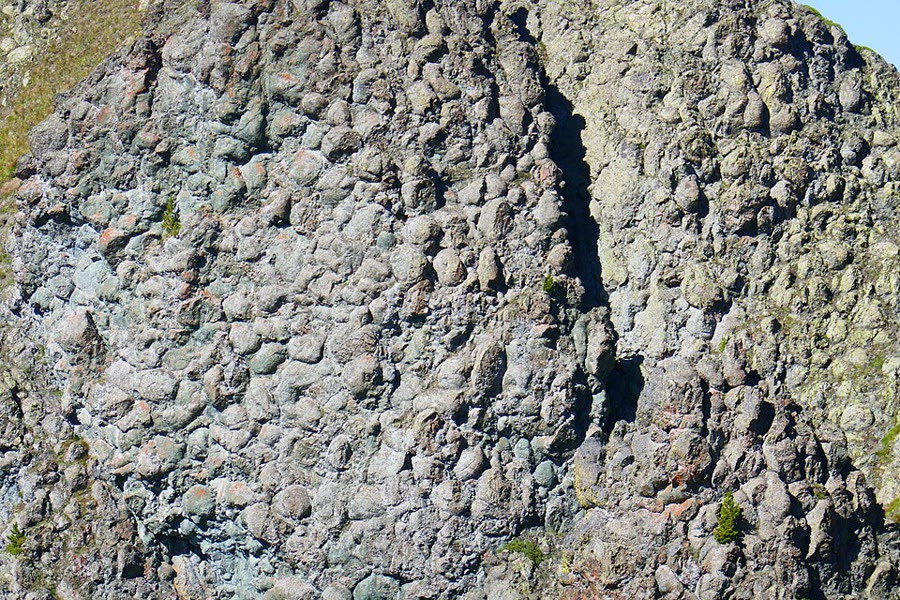
\includegraphics[width=0.66\linewidth]{images/book4/b2-13-pillow-lava.jpg}
\par\smallskip{\small Lavas en almohadilla de la \omterm{def:b2:alpine-orogen:ophiolite}{ofiolita} del Chenaillet, Alpes occidentales: cada almohadilla
redondeada es un lóbulo de basalto que entró en erupción y se enfrió bruscamente en el fondo del océano
Piamonte--Liguria. Fotografía de Lionel Duchoiselle, CC BY-SA 3.0.}
\end{omfigure}

El fondo oceánico puede datarse allí donde cristalizaron sus gabros. Los circones de dos metagabros de
la \omterm{def:b2:alpine-orogen:ophiolite}{ofiolita} de Zermatt--Saas, bajo el Cervino, dan $164.0 \pm \qty{2.7}{Ma}$ y $163.5
\pm \qty{1.8}{Ma}$, y los sedimentos ricos en manganeso depositados sobre los basaltos tienen como mucho $161
\pm \qty{11}{Ma}$: el fondo del océano Piamonte--Liguria se estaba formando en el Jurásico,
hace unos \qty{164}{Myr}.
% ledger: rubatto98:zsf

\section{Subducir un océano, y después un continente}\label{sec:b2:alpine-orogen:subduction}

Un océano se cierra por subducción. Parte de su fondo, sin embargo, acaba encima de un continente
en lugar de debajo, y algunos continentes siguen al océano hacia abajo.

\begin{definition}[Obducción; subducción continental]\label{def:b2:alpine-orogen:obduction}
La \emph{obducción}\index{obducción} es el emplazamiento de una lámina de litosfera oceánica sobre
un margen continental: la \omterm{def:b2:alpine-orogen:ophiolite}{ofiolita} cabalga sobre el continente. La \emph{subducción
continental}\index{subducción continental} es el descenso de litosfera continental, arrastrada
por la placa oceánica que lleva unida, en una zona de subducción después de que se haya consumido el océano
situado delante de ella.
\end{definition}

Hubo \omterm{def:b2:alpine-orogen:obduction}{obducción} en los Dináridos, al sureste de los Alpes: \omterm{def:b2:alpine-orogen:ophiolite}{ofiolitas} del océano jurásico
Vardar, ellas mismas del Jurásico Medio, cabalgaron en el Jurásico Superior sobre una
cuña de acreción y sobre el margen de Apulia. Durante mucho tiempo se pensó que también había emplazado la
\omterm{def:b2:alpine-orogen:ophiolite}{ofiolita} del Chenaillet, porque sus rocas solo muestran un \omterm{def:b2:metamorphic-facies:metamorphism}{metamorfismo} alpino de grado muy
bajo. Un estudio reciente halló relictos de lawsonita y onfacita en su gabro y su
albitita, que sitúan su pico alpino en 10--\qty{11}{kbar} y 340--\qty{360}{\celsius}:
el peso de un \omterm{def:b2:alpine-orogen:nappes}{apilamiento de mantos} de corrimiento de unos 35 a \qty{40}{km} de espesor. Los autores
concluyen que el Chenaillet fue subducido, no obducido, lo que recuerda que la lectura de
una \omterm{def:b2:alpine-orogen:ophiolite}{ofiolita} depende de su historia metamórfica tanto como de sus rocas.
% ledger: schmid04:obduction, corno23:chenaillet

\subsection*{El océano se hunde}

En el Cretácico, el margen meridional, apuliano, del océano Piamonte--Liguria se convirtió en un
margen activo: su fosa se rellenó de lutitas y areniscas, hoy los esquistos calcáreos
llamados Bündnerschiefer o schistes lustrés. Los Alpes orientales registran además una colisión
anterior, el cierre de un golfo de otro océano, el Meliata, contra Apulia, con un
pico de alta presión hacia los \qty{100}{Ma}: los Alpes son el producto de dos orogenias, una
cretácica y otra terciaria.
% ledger: schmid04:two-orogenies

La \omterm{def:b2:alpine-orogen:ophiolite}{ofiolita} de Zermatt--Saas descendió hasta la facies de eclogitas del
\cref{ch:b2:metamorphic-facies}: sus eclogitas alcanzaron 550--\qty{600}{\celsius} y
2.5--\qty{3.0}{GPa}, y el pico de presión se alcanzó entre 48 y \qty{44}{Ma}. Una lámina de ella,
en el Lago di Cignana, contiene coesita y diamantes microscópicos en rocas que empezaron siendo basaltos
y sedimentos del fondo oceánico; alcanzó unos \qty{615}{\celsius} y \qty{2.8}{GPa}, y sus
circones datan ese punto más profundo en $44.1 \pm \qty{0.7}{Ma}$. Un fondo oceánico nacido
hace \qty{164}{Myr} fue subducido, a la edad de 120 millones de años, a profundidades de
\qty{90}{km} o más, y después volvió.
% ledger: halama20:cignana, rubatto98:zsf

\subsection*{El continente lo sigue}

Cuando el océano hubo desaparecido, el margen de Europa fue arrastrado tras él. Las cuarcitas con
coesita del macizo de Dora Maira, vistas en el \cref{ch:b2:pt-paths}, son corteza continental
del lado europeo del océano que llegó a más de \qty{90}{km}, hace unos
\qty{35}{Myr}, y volvió a la velocidad de las placas. Datar las rocas de alta presión
a lo largo de la cordillera da un orden: el propio margen apuliano (la zona de Sesia) en el Cretácico
Superior, las \omterm{def:b2:alpine-orogen:ophiolite}{ofiolitas} del océano Piamonte--Liguria hacia los \qty{44}{Ma}, la
corteza continental europea en el Eoceno superior. Rubatto y colaboradores lo leen como tres episodios de subducción que avanzan en el tiempo de
sureste a noroeste, hacia Europa.
% ledger: chopin84:coesite, rh01:exhumation, rubatto98:zsf, ispra16:cervino

Siguió la colisión: el océano Valais, la última franja oceánica, se cerró durante el Eoceno medio a
superior, y a partir de entonces se apiló corteza continental sobre corteza continental.
La figura siguiente resume la secuencia.
% ledger: schmid04:alpine-tethys

\begin{omfigure}
\centering
\begin{tikzpicture}[x=0.95cm, y=0.78cm, font=\scriptsize]
% (a) rifting and spreading
\begin{scope}[yshift=0cm]
\node[anchor=west, font=\scriptsize\bfseries] at (-0.2,0.75) {(a) Jurásico: se abre el océano};
\fill[gray!25] (0,0) -- (3.2,0) -- (3.8,-0.6) -- (0,-0.6) -- cycle;
\fill[gray!25] (6.2,0) -- (10,0) -- (10,-0.6) -- (5.6,-0.6) -- cycle;
\fill[omThm!35] (3.2,0) -- (6.2,0) -- (5.6,-0.6) -- (3.8,-0.6) -- cycle;
\fill[blue!8] (0,0) rectangle (10,0.4);
\draw[thick] (4.7,0) -- (4.7,-0.6);
\node at (1.6,-0.3) {Europa};
\node at (8,-0.3) {Apulia};
\node[align=center] at (4.7,0.2) {dorsal};
\end{scope}
% (b) oceanic subduction
\begin{scope}[yshift=-1.7cm]
\node[anchor=west, font=\scriptsize\bfseries] at (-0.2,0.75) {(b) Del Cretácico al Eoceno: el océano es subducido};
\fill[blue!8] (0,0) rectangle (7,0.4);
\fill[gray!25] (0,0) -- (3.0,0) -- (3.6,-0.6) -- (0,-0.6) -- cycle;
\fill[omThm!35] (3.0,0) -- (6.3,0) -- (6.0,-0.5) -- (5.6,-0.95) -- (3.6,-0.6) -- cycle;
\fill[gray!25] (6.3,0) -- (6.6,0.3) -- (10,0.3) -- (10,-0.6) -- (6.4,-0.6) -- cycle;
\fill[omThm!35] (5.6,-0.95) -- (6.0,-0.5) -- (7.4,-1.3) -- (7.2,-1.55) -- cycle;
\fill[orange!40] (6.0,0) -- (6.3,0) -- (6.6,0.3) -- (6.35,0.3) -- cycle;
\draw[-{Latex[length=2mm]}] (7.0,-1.0) -- (7.6,-1.38);
\node at (1.6,-0.3) {Europa};
\node at (8.4,-0.15) {Apulia};
\node[anchor=west] at (7.5,-1.1) {eclogita};
\end{scope}
% (c) continental subduction
\begin{scope}[yshift=-3.95cm]
\node[anchor=west, font=\scriptsize\bfseries] at (-0.2,0.75) {(c) Eoceno: el margen europeo lo sigue};
\fill[gray!25] (0,0) -- (5.6,0) -- (6.2,-0.5) -- (7.4,-1.35) -- (7.1,-1.6) -- (5.6,-0.6) -- (0,-0.6) -- cycle;
\fill[omThm!35] (6.2,0.05) -- (6.6,0.3) -- (6.95,0.3) -- (6.4,-0.2) -- cycle;
\fill[gray!25] (6.6,0.3) -- (10,0.3) -- (10,-0.6) -- (6.9,-0.6) -- (6.4,-0.2) -- (6.95,0.3) -- cycle;
\draw[dashed] (6.6,-0.85) circle (0.22);
\draw (6.82,-0.9) -- (7.6,-1.2);
\node[anchor=west] at (7.6,-1.2) {corteza continental UHP};
\node at (2.4,-0.3) {Europa};
\node at (8.4,-0.15) {Apulia};
\end{scope}
% (d) collision
\begin{scope}[yshift=-6.65cm]
\node[anchor=west, font=\scriptsize\bfseries] at (-0.2,1.4) {(d) Del Oligoceno a la actualidad: colisión, mantos de corrimiento, cuencas de antepaís};
\fill[yellow!35] (0.6,0) -- (3.4,0) -- (3.4,-0.3) -- cycle;
\fill[gray!25] (0,-0.3) -- (3.4,-0.3) -- (4.2,0.5) -- (5.2,0.75) -- (6.2,0.55) -- (7.0,0.2) -- (10,0.2)
  -- (10,-0.7) -- (6.6,-0.7) -- (5.4,-1.5) -- (4.0,-1.5) -- (3.2,-0.9) -- (0,-0.9) -- cycle;
\draw (3.4,-0.3) -- (4.5,-1.0);
\draw (4.2,0.5) -- (5.6,-0.4);
\draw (5.2,0.75) -- (6.1,0.1);
\fill[omThm!35] (5.05,0.6) -- (5.55,0.68) -- (5.85,0.32) -- (5.4,0.25) -- cycle;
\fill[yellow!35] (7.0,0.2) -- (9.6,0.2) -- (7.0,-0.1) -- cycle;
\node at (1.4,-0.6) {Europa};
\node at (8.6,-0.3) {Apulia};
\node[anchor=south] at (1.9,0.02) {molasa};
\node at (4.7,-1.25) {raíz};
\node[anchor=south west] at (6.25,0.6) {apilamiento de mantos};
\end{scope}
\end{tikzpicture}
\par\smallskip{\small Historia esquemática de los Alpes, sin escala (litosfera oceánica en rojo,
continental en gris, cuña de acreción en naranja, \omterm{def:b2:alpine-orogen:foreland}{cuencas de antepaís} en amarillo).
(a)~Se abre el océano Piamonte--Liguria entre Europa y Apulia. (b)~Su fondo es subducido
bajo Apulia y convertido en eclogita. (c)~El margen europeo es arrastrado tras él y
metamorfizado a ultra alta presión. (d)~La corteza continental se apila en \omterm{def:b2:alpine-orogen:nappes}{mantos de corrimiento} sobre una
raíz engrosada, con \omterm{def:b2:alpine-orogen:foreland}{cuencas de antepaís} flexurales a ambos lados.}
\end{omfigure}
% ledger: schmid04:alpine-tethys, schmid04:two-orogenies, rubatto98:zsf, schmid04:foreland

\section{Mantos de corrimiento, klippes y ventanas}\label{sec:b2:alpine-orogen:nappes}

Los fragmentos de océano y de continente no se apilaron enteros. Fueron arrancados en finas
láminas y transportados lejos.

\begin{definition}[Manto de corrimiento; apilamiento de mantos]\label{def:b2:alpine-orogen:nappes}
Un \emph{manto de corrimiento}\index{manto de corrimiento} es una gran lámina de roca, a menudo de unos pocos kilómetros de espesor y decenas
de kilómetros de longitud, transportada a lo largo de un cabalgamiento de bajo ángulo o en el flanco invertido de un gran
pliegue tumbado lejos de su lugar de origen; las rocas de un manto de corrimiento son
\emph{alóctonas}\index{alóctono (unidad de roca)}, y las que se quedaron en su sitio,
\emph{autóctonas}\index{autóctono (unidad de roca)}. Un \emph{apilamiento de
mantos}\index{apilamiento de mantos} es una pila de mantos de corrimiento en la que los mantos estructuralmente más altos
proceden por lo general de zonas más internas del \omterm{def:b2:alpine-orogen:orogen}{orógeno}.
\end{definition}

En los Alpes, el orden de apilamiento es la geografía del océano desaparecido puesta del revés,
y las unidades reciben el nombre de su origen (tabla siguiente).

\begin{omfigure}
\centering\small
\begin{tabular}{>{\raggedright\arraybackslash}p{0.24\linewidth}|>{\raggedright\arraybackslash}p{0.66\linewidth}}
unidad (de techo a muro) & origen y rocas \\ \hline
mantos austroalpinos & margen de Apulia al norte de la Línea Periadriática: zócalo y láminas
de cobertera despegadas de su corteza inferior \\
mantos de Margna--Sesia (zona de Sesia, Dent Blanche) & fragmentos separados por el rift del margen
apuliano más externo cuando se abrió el océano \\
mantos penínicos superiores & océano Piamonte--Liguria: \omterm{def:b2:alpine-orogen:ophiolite}{ofiolitas}, manto exhumado, esquistos
calcáreos \\
mantos penínicos medios & el continente en cinta brianzonés \\
mantos penínicos inferiores & océano Valais: \omterm{def:b2:alpine-orogen:ophiolite}{ofiolitas} y esquistos calcáreos \\
mantos subpenínicos & zócalo europeo despegado de su corteza inferior \\
mantos helvéticos & cobertera rica en calizas del margen europeo próximo, despegada de su
zócalo \\ \hline
Alpes Meridionales & Apulia al sur de la Línea Periadriática: un \omterm{def:b2:alpine-orogen:ftb}{cinturón de pliegues y cabalgamientos} de vergencia sur,
sobre todo mioceno, de 10 a \qty{15}{km} de espesor
\end{tabular}
\par\smallskip{\small Las principales unidades tectónicas de los Alpes, desde el techo estructural
hacia abajo, con el dominio del que procede cada una (según Schmid y colaboradores).}
\end{omfigure}
% ledger: schmid04:units, schmid04:apulia

La placa superior, Apulia, está arriba; debajo vienen, por orden, el océano lejano, el
Brianzonés, el océano próximo y el margen europeo, y las unidades más bajas son las que
estaban más cerca de Europa. Grandes pliegues que replegaron los \omterm{def:b2:alpine-orogen:nappes}{mantos de corrimiento} después de su apilamiento
alteran a veces el orden, y algunas franjas, como el Brianzonés, se acuñan a lo largo de
la cordillera.
% ledger: schmid04:units, schmid04:alpine-tethys

La erosión corta después el apilamiento, y en un mapa aparecen dos formas.

\begin{definition}[Klippe; ventana tectónica]\label{def:b2:alpine-orogen:klippe}
Un \emph{klippe}\index{klippe} (plural klippes) es un resto aislado de un \omterm{def:b2:alpine-orogen:nappes}{manto de corrimiento} que
ha quedado sobre las rocas de debajo cuando la erosión ha eliminado el resto de la lámina; está
rodeado por su cabalgamiento basal. Una \emph{ventana tectónica}\index{ventana tectónica} es un agujero
abierto por la erosión a través de un \omterm{def:b2:alpine-orogen:nappes}{manto de corrimiento}, donde afloran las rocas situadas bajo su cabalgamiento basal, rodeado por el
manto.
\end{definition}

\begin{omfigure}
\centering
\begin{tikzpicture}[x=0.68cm, y=0.68cm, font=\scriptsize]
\def\thrust{(0,0) -- (5,0) .. controls (6.5,0) and (7,1.1) .. (8,1.1)
  .. controls (9,1.1) and (9.5,0) .. (11,0) -- (16,0)}
\def\topo{(0,1.7) .. controls (3,1.9) and (5,1.8) .. (6,1.5) .. controls (7,1.0) .. (8,0.6)
  .. controls (9,1.0) .. (10.3,1.5) .. controls (11.3,1.3) .. (12.5,-0.4)
  .. controls (13.3,0.9) .. (14.5,0.95) .. controls (15.5,0.8) .. (16,-0.2)}
\begin{scope}
\clip \topo -- (16,-2.6) -- (0,-2.6) -- cycle;
\fill[gray!20] (0,-2.6) rectangle (16,2.2);
\fill[omThm!30] \thrust -- (16,2.2) -- (0,2.2) -- cycle;
\draw[gray!55, yshift=-0.9*0.68cm] \thrust;
\draw[gray!55, yshift=-1.8*0.68cm] \thrust;
\draw[line width=1.2pt] \thrust;
\end{scope}
\draw \topo;
\node at (2.5,1.0) {manto};
\node[anchor=north west] at (0.2,-0.05) {cabalgamiento basal};
\node at (3.6,-1.35) {autóctono};
\draw[-{Latex[length=1.6mm]}] (8,2.0) node[anchor=south] {ventana tectónica} -- (8,0.75);
\draw[-{Latex[length=1.6mm]}] (14.5,2.0) node[anchor=south] {klippe} -- (14.5,1.05);
\end{tikzpicture}
\par\smallskip{\small Un \omterm{def:b2:alpine-orogen:nappes}{manto de corrimiento} (en color) sobre su autóctono (gris) tras la erosión, en un
corte esquemático: donde su cabalgamiento basal (trazo grueso) se arquea hacia arriba, la erosión ha atravesado
el manto y ha abierto una \omterm{def:b2:alpine-orogen:klippe}{ventana tectónica} sobre las rocas de debajo; por delante, un resto del
manto queda aislado sobre el autóctono: un \omterm{def:b2:alpine-orogen:klippe}{klippe}.}
\end{omfigure}

Los Alpes están llenos de ambos. El Cervino es un \omterm{def:b2:alpine-orogen:klippe}{klippe}: su cima pertenece al sistema de cabalgamientos de la Dent
Blanche, un cerro testigo de rocas apulianas situado encima de toda la cuña, con
gneises y gabros de edad pérmica que descansan sobre las \omterm{def:b2:alpine-orogen:ophiolite}{ofiolitas} del manto de Zermatt--Saas
y la zona del Combin, que descansan a su vez sobre los mantos del Monte Rosa y del Gran San Bernardo, del
lado europeo (fotografía siguiente). En el frente septentrional de los
Alpes occidentales, mantos de cobertera procedentes de zonas muy internas de la cordillera forman los Prealpes romandos y los
\omterm{def:b2:alpine-orogen:klippe}{klippes} de Suiza central. En los Alpes orientales se abren dos ventanas a través de la tapa
austroalpina: la ventana de la Engadina, donde los esquistos del océano Valais con esquistos azules aparecen
bajo los últimos restos del Brianzonés, y la ventana de los Tauern, más grande, donde el
margen europeo y láminas del Tetis alpino salen de debajo de los mantos
austroalpinos.
% ledger: ispra16:cervino, schmid04:windows

\begin{omfigure}
\centering
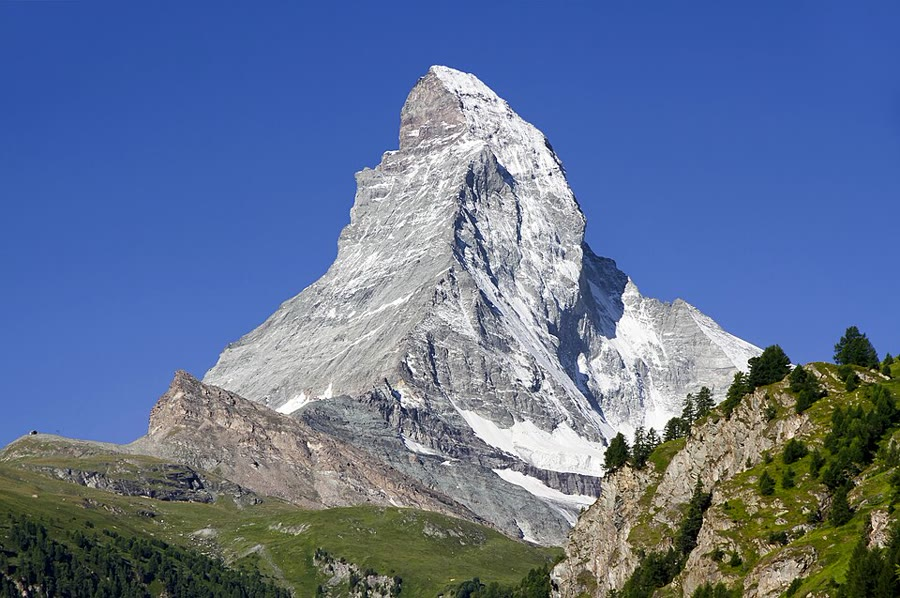
\includegraphics[width=0.7\linewidth]{images/book4/b2-13-matterhorn.jpg}
\par\smallskip{\small La cara nordeste del Cervino (\qty{4478}{m}), vista desde Zermatt:
su pirámide superior es gneis y gabro apulianos del sistema de cabalgamientos de la Dent Blanche, un \omterm{def:b2:alpine-orogen:klippe}{klippe}
sobre las \omterm{def:b2:alpine-orogen:ophiolite}{ofiolitas} del Tetis alpino. Fotografía de Ximonic (Simo Räsänen), CC BY-SA
4.0.}
\end{omfigure}
% ledger: ispra16:cervino

\subsection*{Los despegues y las dos pieles}

Los \omterm{def:b2:alpine-orogen:nappes}{mantos de corrimiento} y las láminas cabalgantes se desplazan sobre superficies de debilidad.

\begin{definition}[Despegue]\label{def:b2:alpine-orogen:decollement}
Un \emph{despegue}\index{despegue} (\textit{décollement}) es una superficie de bajo ángulo a lo largo de la cual una
serie de rocas se separa de las de debajo y se desliza sobre ellas, deformándose ambos lados
de forma independiente; suele seguir una capa débil, como una evaporita o una lutita.
\end{definition}

\begin{definition}[Tectónica de piel fina y tectónica de piel gruesa]\label{def:b2:alpine-orogen:skin}
La \emph{tectónica de piel fina}\index{tectónica de piel fina} es la deformación de una
cobertera sedimentaria despegada de su zócalo a lo largo de un \omterm{def:b2:alpine-orogen:decollement}{despegue} basal: la cobertera se pliega y
cabalga mientras el zócalo de debajo permanece sin deformar. La \emph{tectónica de piel
gruesa}\index{tectónica de piel gruesa} es la deformación en la que interviene el zócalo:
cobertera y zócalo se acortan juntos sobre fallas que penetran en el zócalo.
\end{definition}
% ledger: lanza22:jura

\begin{definition}[Cinturón de pliegues y cabalgamientos]\label{def:b2:alpine-orogen:ftb}
Un \emph{cinturón de pliegues y cabalgamientos}\index{cinturón de pliegues y cabalgamientos} es una franja de pliegues y fallas de cabalgamiento
que acorta la parte externa de un \omterm{def:b2:alpine-orogen:orogen}{orógeno} y se propaga hacia su antepaís; los cabalgamientos
suben en escalón desde el \omterm{def:b2:alpine-orogen:decollement}{despegue} a través de las capas, y los pliegues crecen sobre ellos.
\end{definition}

Los Alpes tienen las dos pieles. Los mantos helvéticos son un \omterm{def:b2:alpine-orogen:ftb}{cinturón de pliegues y cabalgamientos} de piel fina: las
calizas mesozoicas del margen europeo próximo despegadas de su zócalo. Su base es
el cabalgamiento de Glaris, donde capas rojas pérmicas descansan sobre \omterm{def:b2:alpine-orogen:foreland}{flysch} cenozoico. En el Mioceno, en
cambio, bloques de zócalo de los macizos externos, zócalo europeo acortado y engrosado (los macizos del
Aar, el Mont Blanc, Belledonne, el Pelvoux y el Argentera), cabalgaron hacia arriba con su
cobertera: un cabalgamiento de piel gruesa.
% ledger: schmid04:units, schmid04:skins, herwegh08:glarus, rosenberg21:massifs

El Jura, el arco de crestas al noroeste de la llanura suiza, es el ejemplo clásico de piel
fina. En el Mioceno superior y el Plioceno su cobertera mesozoica se plegó y cabalgó sobre un
\omterm{def:b2:alpine-orogen:decollement}{despegue} situado en las débiles evaporitas del Triásico Medio y Superior, mientras que el zócalo de
debajo, que continúa desde los macizos externos bajo la cuenca de la \omterm{def:b2:alpine-orogen:foreland}{Molasa}, no intervino: según
la lectura clásica, el empuje venía de los lejanos macizos externos. La sismología ha añadido después
un capítulo de piel gruesa. Los terremotos de Saint-Ursanne de 2000 tuvieron su foco a
menos de un kilómetro de profundidad y un mecanismo de cabalgamiento, un cabalgamiento activo y somero en la cobertera,
mientras que otros estudios hallan fallas de zócalo reactivadas desde el Plioceno más tardío. Si
el Jura sigue despegado de su zócalo es objeto de debate.
% ledger: lanza22:jura, schmid04:skins

\begin{inthefield}[Leer un contacto de cabalgamiento]
Entre Flims y el Walensee, en el este de Suiza, discurre el cabalgamiento de Glaris, uno de los
grandes cabalgamientos de bajo ángulo más destacados de los Alpes. A lo largo de él, capas rojas pérmicas, el
Verrucano, descansan sobre \omterm{def:b2:alpine-orogen:foreland}{flysch} cenozoico: rocas mucho más antiguas sobre otras más jóvenes. Entre ambas, una
banda delgada y fuertemente cizallada de caliza forma el contacto: la caliza de Lochseiten, en la que se concentró el desplazamiento, de al menos 30 a
\qty{40}{km}. En el siglo XIX Heim interpretó la estructura como dos enormes
pliegues tumbados enfrentados; Escher von der Linth había visto en ella un único cabalgamiento, y la interpretación como cabalgamiento se impuso. Un geólogo que encuentra un contacto así comprueba
tres cosas: si hay rocas más antiguas sobre otras más jóvenes, algo que ninguna estratificación normal puede producir;
si las capas de ambos lados quedan cortadas en el contacto; y si el propio contacto
es una banda de roca cizallada y recristalizada más que un plano de estratificación.
\end{inthefield}
% ledger: herwegh08:glarus

\section{Las cuencas de antepaís: flysch y molasa}\label{sec:b2:alpine-orogen:foreland}

Una cordillera carga la placa sobre la que se apoya, y la placa se flexiona hacia abajo delante de ella.

\begin{definition}[Cuenca de antepaís; flysch; molasa]\label{def:b2:alpine-orogen:foreland}
Una \emph{cuenca de antepaís}\index{cuenca de antepaís} es una cuenca sedimentaria alargada que se forma
entre un \omterm{def:b2:alpine-orogen:orogen}{orógeno} y el continente estable situado delante de él, donde la placa se flexiona hacia abajo bajo
la carga de la cuña de cabalgamientos; es más profunda junto al frente de cabalgamiento y es a su vez
cabalgada progresivamente. El \emph{flysch}\index{flysch} es el relleno de aguas profundas de esa
cuenca, sobre todo turbiditas de arenisca y lutita depositadas mientras la cuenca está subalimentada.
La \emph{molasa}\index{molasa} es su relleno posterior, marino somero y continental, sobre todo
conglomerados y areniscas procedentes de la erosión de la cordillera, depositados una vez que el aporte colma la
cuenca.
\end{definition}
% ledger: sinclair97:trinity, schmid04:foreland, krenmayr99:molasse

La flexión es una flexura elástica de la litosfera, tratada en un capítulo del volumen de tercer
año; aquí solo importa su efecto sobre la cuenca. Sinclair describió la primera \omterm{def:b2:alpine-orogen:foreland}{cuenca de antepaís} alpina, de edad paleocena a oligocena,
como una «trinidad subalimentada»: calizas en el lado continental, fango hemipelágico en el
centro, turbiditas de aguas profundas contra el frente de cabalgamiento. A medida que avanzaban los cabalgamientos, la cuenca
se desplazaba con ellos: a través de Suiza su línea de costa continental avanzó hacia el noroeste a razón de 8.5
a \qty{12.9}{mm} al año, y la cuenca migró con una forma casi constante a lo largo de al menos
\qty{210}{km} sobre la placa europea.
% ledger: sinclair97:trinity

La cuenca de la \omterm{def:b2:alpine-orogen:foreland}{Molasa} del norte de los Alpes, que se extiende desde los Alpes Marítimos hasta Viena, empezó a
subsidir en el Eoceno superior. El \omterm{def:b2:alpine-orogen:foreland}{flysch} del Oligoceno inferior, que hoy se encuentra encima de los mantos
helvéticos, registra una última etapa de aguas profundas; desde el Oligoceno superior hasta el Mioceno superior, los ríos
extendieron gravas y arenas continentales procedentes de las jóvenes montañas. El nombre es antiguo: H.-B. de Saussure
introdujo \emph{molasse} en 1779. El relleno se engruesa hacia la cordillera: en el
sector austriaco, hasta más de \qty{4000}{m} en el frente de cabalgamiento, y en otras partes de la cuenca
una sola serie de conglomerados fluviales del Oligoceno superior tiene unos \qty{4}{km} de espesor. La parte meridional de
la cuenca ha sido cabalgada: la franja de afloramientos austriaca, de unos \qty{60}{km} de ancho, es menos
de la cuarta parte de la anchura que tenía la cuenca. La propia \omterm{def:b2:alpine-orogen:foreland}{molasa} cabalgada ha quedado atrapada en
los cabalgamientos como \omterm{def:b2:alpine-orogen:foreland}{Molasa} Subalpina, láminas de conglomerado buzantes al sur a lo largo del
borde septentrional de la cordillera.
% ledger: schmid04:foreland, krenmayr99:molasse, gs18:conglomerates

Al sur de los Alpes, la llanura del Po descansa sobre el antepaís adriático, poco deformado, de los
Alpes Meridionales. Sus sedimentos más jóvenes, pliocenos y pleistocenos, recubren en parte estructuras alpinas
en discordancia y en parte están deformados por los últimos cabalgamientos de los Alpes Meridionales
y de los Apeninos.
% ledger: schmid04:foreland

\begin{omfigure}
\centering
\begin{tikzpicture}[x=0.5cm, y=0.6cm, font=\scriptsize]
\begin{scope}
\node[anchor=west, font=\scriptsize\bfseries] at (0,2.4) {(a) subalimentada: flysch};
\fill[blue!8] (0,0) -- (12,0) -- (12,1.4) -- (9.0,1.4) -- (4,0.05) -- (0,0.05) -- cycle;
\fill[gray!25] (0,0) -- (12,-1.1) -- (12,-1.9) -- (0,-0.8) -- cycle;
\fill[omThm!30] (9.0,1.4) -- (12,2.2) -- (12,-1.1) -- (9.5,-0.87) -- cycle;
\fill[green!25!gray!40] (5.5,-0.5) -- (9.5,-0.87) -- (9.3,-0.35) -- (7.0,-0.2) -- cycle;
\node at (10.9,0.6) {cuña};
\node at (2,-0.45) {cratón};
\node[anchor=north] at (7.3,-0.9) {turbiditas};
\draw[->] (7.3,-0.95) -- (7.6,-0.55);
\end{scope}
\begin{scope}[xshift=6.4cm]
\node[anchor=west, font=\scriptsize\bfseries] at (0,2.4) {(b) sobrealimentada: molasa};
\fill[gray!25] (0,0) -- (12,-1.1) -- (12,-1.9) -- (0,-0.8) -- cycle;
\fill[omThm!30] (8.5,1.6) -- (12,2.4) -- (12,-1.1) -- (9.0,-0.82) -- cycle;
\fill[yellow!40] (1.5,-0.13) -- (9.0,-0.82) -- (8.5,1.0) -- (5,0.35) -- cycle;
\fill[blue!8] (0,0) -- (1.5,-0.13) -- (5,0.35) -- (4,0.4) -- (0,0.4) -- cycle;
\node at (10.6,0.6) {cuña};
\node at (2,-0.45) {cratón};
\node at (6.2,-0.05) {gravas, arenas};
\end{scope}
\end{tikzpicture}
\par\smallskip{\small Una \omterm{def:b2:alpine-orogen:foreland}{cuenca de antepaís} en dos etapas (esquema). (a)~Al principio, la placa
flexionada subside más deprisa de lo que llega el sedimento: aguas profundas contra la cuña de cabalgamientos, donde
se acumulan turbiditas (\omterm{def:b2:alpine-orogen:foreland}{flysch}). (b)~Más tarde, la cordillera en erosión aporta más de lo que la cuenca puede
contener: los ríos la rellenan de gravas y arenas (\omterm{def:b2:alpine-orogen:foreland}{molasa}), y la cuña cabalga sobre sus propios
derrubios.}
\end{omfigure}
% ledger: sinclair97:trinity, schmid04:foreland

\section{Leer la historia: cortes y geofísica}\label{sec:b2:alpine-orogen:sections}

Un mapa muestra dónde están las unidades; un corte muestra cómo se disponen en profundidad, y puede
ponerse a prueba.

\begin{definition}[Corte compensado]\label{def:b2:alpine-orogen:balanced}
Un \emph{corte compensado}\index{corte compensado} es un corte geológico de rocas deformadas,
trazado paralelo a la dirección de transporte, que puede restituirse a un estado no deformado geológicamente
razonable sin ganar ni perder roca: las longitudes de las capas guía y
las áreas de las unidades de roca del corte se conservan entre el estado deformado y el
restituido.
\end{definition}

La restitución se ancla en \emph{líneas de referencia} (\textit{pin lines}), líneas que atraviesan las capas en los extremos del
corte, elegidas donde las rocas no se deslizaron unas respecto de otras.

\begin{proposition}[Compensación de longitudes y de áreas]\label{prop:b2:alpine-orogen:balance}
Entre dos líneas de referencia separadas una distancia $l$ en el estado deformado, sea una capa guía de
longitud $l_0$ medida a lo largo de la capa, y sea una capa de espesor original $t$ de
área $A$ en el corte. Si la longitud y el área se conservan en el plano del corte,
\begin{enumerate}
\item la capa medía $l_0$ antes de la deformación, el acortamiento es
$e = 1 - l/l_0$ y la distancia de acortamiento es $S = l_0 - l$;
\item la longitud restituida de la capa es $l_0 = A/t$;
\item si un horizonte guía estaba a una profundidad $d$ sobre un \omterm{def:b2:alpine-orogen:decollement}{despegue} plano, el área de roca
elevada por encima del nivel original del horizonte, su \emph{área en exceso} $A_e$, es igual a $S\,d$;
por tanto $d = A_e/S$.
\end{enumerate}
\end{proposition}

\begin{omfigure}
\centering
% book's own geometry (figdata/bachelor-2/alps.py)
\begin{tikzpicture}
\begin{axis}[width=0.86\linewidth, height=4.0cm, axis equal image, xmin=-1.5, xmax=31.5,
  ymin=-7.5, ymax=4.8, axis lines=none, clip=false]
\addplot[omThm, line width=1.2pt] table[x=x_km, y=y_km] {figdata/out/bachelor-2-alps-chevron.dat};
\addplot[gray, line width=1.2pt] table[x=x_km, y=y_km] {figdata/out/bachelor-2-alps-chevron0.dat};
\draw[dashed] (axis cs:0,-7) -- (axis cs:0,4.3);
\draw[dashed] (axis cs:22.98,-1.2) -- (axis cs:22.98,4.3);
\draw[dashed] (axis cs:30,-7) -- (axis cs:30,-4.8);
\draw[<->] (axis cs:0,-1.4) -- node[below, font=\scriptsize] {$l = \qty{23.0}{km}$} (axis cs:22.98,-1.4);
\node[font=\scriptsize, anchor=south] at (axis cs:15,-5.9) {restituida: $l_0 = \qty{30.0}{km}$};
\node[font=\scriptsize, anchor=west] at (axis cs:23.3,2.2) {buzamiento de los flancos \qty{40}{\degree}};
\node[font=\scriptsize, anchor=south] at (axis cs:0,4.3) {referencia};
\node[font=\scriptsize, anchor=south] at (axis cs:22.98,4.3) {referencia};
\end{axis}
\end{tikzpicture}
\par\smallskip{\small Compensación de longitudes de una capa guía plegada en chevrones con flancos
buzantes \qty{40}{\degree} (arriba), y la misma capa restituida entre sus líneas de referencia
(abajo), a escala real. Cada flanco conserva su longitud; la capa plegada abarca
$l = 30.0\cos\qty{40}{\degree} = \qty{23.0}{km}$, un acortamiento de $1 - \cos\qty{40}{\degree} =
\qty{23.4}{\percent}$.}
\end{omfigure}

\begin{proof}
(1) Una capa que no se estira ni se acorta a lo largo de su longitud la conserva; el acortamiento es
la fracción de longitud perdida, como en la escuela. (2) Antes de la deformación la capa es una franja de
longitud $l_0$ y espesor $t$, de área $l_0 t$, y el área se conserva. (3) Antes de la
deformación, la roca entre el nivel del horizonte guía y el \omterm{def:b2:alpine-orogen:decollement}{despegue} ocupaba una franja de $l_0$
de longitud y $d$ de espesor. Después, entre las líneas de referencia, la misma roca ocupa una franja de $l$ de longitud
desde el \omterm{def:b2:alpine-orogen:decollement}{despegue} hasta el nivel original del horizonte, de área $l\,d$, más el área
en exceso empujada por encima de ese nivel. La conservación da $l_0 d = l\,d + A_e$, de modo que $A_e = (l_0 -
l)\,d = S\,d$. La relación da la profundidad de un \omterm{def:b2:alpine-orogen:decollement}{despegue} oculto a partir de un área en exceso
y un acortamiento medidos.
\end{proof}


\begin{method}[Restituir un corte]\label{met:b2:alpine-orogen:restore}
\begin{enumerate}
\item Elíjase un corte paralelo a la dirección de transporte y dos líneas de referencia donde no
hubo deslizamiento entre capas.
\item Mídase cada capa guía a lo largo de su longitud entre las referencias, contando cada tramo
repetido por un cabalgamiento.
\item Extiéndanse las capas en horizontal con sus longitudes medidas, conservando el orden de las capas,
y vuélvanse a dibujar las fallas en el corte restituido: sus truncaciones deben coincidir, sin huecos
ni solapamientos.
\item Compárese: las capas de una misma lámina cabalgante deben restituirse a la misma longitud; las áreas de
las capas, divididas por sus espesores, deben dar también las mismas longitudes. Un corte que
no lo cumple no es admisible tal como está dibujado.
\end{enumerate}
\end{method}

La compensación es una prueba de un corte, no una demostración, y sus hipótesis importan. En el Jura,
cerca del Chasseral, la compensación de longitudes del techo del Jurásico da \qty{5.1}{km} de
desplazamiento, pero la compensación de áreas y la modelización directa dan \qty{11.3}{km}: los
\qty{6.2}{km} adicionales se transmitieron a lo largo de un segundo \omterm{def:b2:alpine-orogen:decollement}{despegue}, superior, en las lutitas jurásicas, y pasaron
a pliegues situados más al norte. Una sola capa guía había pasado por alto la mitad del movimiento. El mismo estudio
sopesó, sin necesitarlas, otras dos interpretaciones habituales en el Jura: altos de zócalo que empujan
hacia arriba los pliegues, y núcleos de anticlinal engrosados por evaporitas triásicas que fluyen hacia ellos, un
proceso que invalida la compensación de áreas, ya que la capa de evaporitas deja de conservar su
espesor.
% ledger: schori15:chasseral, schori15:evaporite-flow

\subsection*{¿Cuánto acortamiento?}

Aplicada a transectas completas, la compensación da el acortamiento total de la cordillera, y las respuestas
varían con las hipótesis. A través de los Alpes Centrales, a lo largo de la transecta NFP-20, las estimaciones
del acortamiento colisional han sido de unos \qty{125}{km} en trabajos anteriores, \qty{160}{km} en
una compilación de 2015 y \qty{144}{km} en una revisión de 2021; añadir el desplazamiento dextro de la Línea Periadriática, que
movió Apulia lateralmente a lo largo de la cordillera, eleva la convergencia total a entre 206 y
\qty{250}{km}, según cuánto desplazamiento se suponga. En los Alpes occidentales las estimaciones
van de 124 a \qty{243}{km}. Cada una de ellas es una suma de piezas restituidas, cada una con
sus propias líneas de referencia y sus propias conjeturas sobre lo que eliminaron la erosión y la subducción.
% ledger: rosenberg21:shortening

\subsection*{Lo que ve la geofísica}

Los cortes en profundidad se apoyan en la geofísica. Se han realizado perfiles de sísmica de reflexión profunda
a través de la cordillera (ECORS--CROP en los Alpes occidentales, NFP-20 Oeste y Este en
Suiza, TRANSALP en el este), y densas redes de sismómetros cartografían hoy el Moho
a partir de funciones receptoras, las conversiones de ondas P telesísmicas en ondas S en la base de
la corteza. El mapa de AlpArray, construido con más de cien mil funciones receptoras,
sitúa el Moho a unos \qty{30}{km}, lo típico de los continentes, alrededor de la cordillera, y a 55--\qty{60}{km}
bajo los Alpes; el Moho europeo buza suavemente desde unos \qty{30}{km} en el
noroeste hasta unos \qty{55}{km} bajo la cordillera.
El corte esquemático siguiente resume cómo se interpretan los perfiles NFP-20 a través de los Alpes
Centrales.
% ledger: schmid04:transects, michailos23:moho

\begin{omfigure}
\centering
\begin{tikzpicture}[x=0.6cm, y=0.5cm, font=\scriptsize]
% surface and cover
\fill[yellow!30] (0,0) -- (3.0,0) -- (6.5,-0.3) -- (8.0,0.4) -- (8.0,-0.9) -- (0,-0.6) -- cycle;
\fill[gray!12] (0,-0.6) -- (8.0,-0.9) -- (12.5,-4.5) -- (15,-3.5) -- (16.5,-6.6) -- (16,-8.3)
  -- (0,-5.0) -- cycle;
\fill[gray!35] (0,-5.0) -- (16,-8.3) -- (17.5,-10.0) -- (0,-6.0) -- cycle;
% Helvetic and Aar
\fill[cyan!25] (8.0,0.4) -- (10.0,1.6) -- (11.0,1.2) -- (9.5,-0.4) -- (8.0,-0.9) -- cycle;
\fill[gray!12] (8.0,-0.9) -- (9.5,-0.4) -- (11.0,1.2) -- (12.0,2.0) -- (12.8,0.2) -- (11.5,-1.8)
  -- (12.5,-4.5) -- cycle;
% Penninic stack
\fill[omThm!35] (12.0,2.0) -- (14.5,2.6) -- (17.0,2.2) -- (17.3,-1.0) -- (15.0,-3.5) -- (12.5,-4.5)
  -- (11.5,-1.8) -- (12.8,0.2) -- cycle;
% Austroalpine/Apulia and Southern Alps
\fill[orange!30] (17.0,2.2) -- (19.0,1.6) -- (24,0.2) -- (26,0) -- (26,-3.5) -- (20.5,-4.0)
  -- (17.3,-1.0) -- cycle;
\fill[brown!35] (17.3,-1.0) -- (20.5,-4.0) -- (19.0,-7.0) -- (16.5,-6.6) -- (15,-3.5) -- cycle;
\fill[gray!35] (20.5,-4.0) -- (26,-3.5) -- (26,-6.0) -- (19.0,-7.0) -- cycle;
\fill[yellow!30] (23.5,0.3) -- (26,0) -- (26,-0.5) -- (24.5,-0.3) -- cycle;
\draw[thick] (17.3,-1.0) -- (17.0,2.2);
\draw[thick] (8.0,-0.9) -- (12.5,-4.5);
\draw[dashed] (0,-6.0) -- (17.5,-10.0);
\draw[dashed] (19.0,-7.0) -- (26,-6.0);
\node at (2.2,-0.25) {Jura};
\node at (5.2,-0.35) {molasa};
\node at (9.0,0.15) {Helvético};
\node at (10.6,-0.6) {Aar};
\node at (14.6,0.4) {mantos penínicos};
\node at (21.2,-0.9) {Alpes Meridionales};
\node at (24.9,-0.3) {Po};
\node at (18.0,-4.8) {Ivrea};
\node[align=center] at (5,-3.0) {corteza europea};
\node[anchor=north] at (3.2,-7.4) {Moho europeo};
\node at (10,-9.3) {manto};
\node at (23,-7.7) {manto};
\node[anchor=north] at (23,-6.55) {Moho adriático};
\node[anchor=south, align=center] at (17.2,2.25) {Línea\\Periadriática};
\draw[-{Latex[length=2mm]}] (1.0,0.5) -- (0.0,0.5);
\node[anchor=south] at (0.5,0.5) {NO};
\draw[-{Latex[length=2mm]}] (25.0,1.2) -- (26.0,1.2);
\node[anchor=south] at (25.5,1.2) {SE};
\end{tikzpicture}
\par\smallskip{\small Corte cortical esquemático a través de los Alpes Centrales, desde el Jura hasta
la llanura del Po (sin escala; según las interpretaciones de las transectas NFP-20 recopiladas por
Schmid y colaboradores). La corteza europea, con el Jura plegado y despegado de su techo, se hunde bajo
los mantos helvéticos, el macizo del Aar y el \omterm{def:b2:alpine-orogen:nappes}{apilamiento de mantos} penínicos; al sur de la Línea
Periadriática, la corteza apuliana con la cuña del cuerpo de Ivrea se sitúa sobre el Moho europeo, y los
Alpes Meridionales cabalgan hacia el sur sobre la llanura del Po.}
\end{omfigure}
% ledger: schmid04:transects, schmid04:units, schmid04:apulia, schmid04:skins


\begin{omfigure}
\centering
% ledger: data:b4-etopo-alps, data:b4-alps-moho, michailos23:moho
\begin{tikzpicture}
\begin{groupplot}[group style={group size=1 by 2, vertical sep=0.25cm, x descriptions at=edge bottom},
  width=0.92\linewidth, xmin=0, xmax=300, tick label style={font=\scriptsize},
  label style={font=\small}]
\nextgroupplot[height=3.6cm, ymin=0, ymax=4000, ylabel={altitud (\unit{m})},
  ytick={0,1000,2000,3000,4000}, y tick label style={/pgf/number format/1000 sep={}},
  legend style={font=\scriptsize, at={(0.99,0.97)}, anchor=north east, draw=none, fill=none}]
\addplot[gray, line width=0.4pt] table[x=km, y=max_m] {figdata/out/bachelor-2-alps-swath.dat};
\addplot[omThm, line width=1pt] table[x=km, y=mean_m] {figdata/out/bachelor-2-alps-swath.dat};
\legend{máximo de la franja, media de la franja}
\node[font=\scriptsize, anchor=south west] at (axis cs:2,2650) {A (llanura del Po)};
\node[font=\scriptsize, anchor=south east] at (axis cs:298,1500) {B};
\nextgroupplot[height=4.6cm, ymin=0, ymax=70, y dir=reverse, xlabel={distancia al norte de
  \qty{45.3}{\degree} N a lo largo de \qty{8}{\degree} E (\unit{km})}, ylabel={profundidad (\unit{km})},
  legend style={font=\scriptsize, at={(0.99,0.03)}, anchor=south east, draw=none, fill=none}]
\addplot[only marks, mark=*, mark size=1.6pt, black] table[x=km, y=moho_km] {figdata/out/bachelor-2-alps-moho.dat};
\addplot[omThm, dashed, line width=0.8pt] table[x=km, y=airy_km] {figdata/out/bachelor-2-alps-airy.dat};
\addplot[gray, densely dotted] coordinates {(0,30) (300,30)};
\legend{Moho observado, predicción de Airy, \qty{30}{km}}
\end{groupplot}
\end{tikzpicture}
\par\smallskip{\small Perfil A--B a lo largo de \qty{8}{\degree} E. Arriba: altitud media y máxima
de los nodos de ETOPO1 en una franja de \qty{0.25}{\degree} a cada lado del meridiano.
Abajo: las profundidades del Moho determinadas sobre este meridiano en el mapa de funciones receptoras de AlpArray
(Michailos y colaboradores, CC BY 4.0), y el Moho que la isostasia local de Airy situaría bajo
el relieve medio de la franja, para una corteza de \qty{30}{km} y densidades de 2700 y
\qty{3300}{kg.m^{-3}}.}
\end{omfigure}

El perfil anterior confronta la raíz con el modelo de Airy del volumen de primer
año. Bajo la parte más alta del perfil, donde el relieve medio de la franja alcanza
\qty{2.74}{km} a \qty{46.5}{\degree} N, una raíz de Airy local situaría el Moho a
$30 + 4.5 \times 2.74 = \qty{42.3}{km}$; se observa a \qty{36.3}{km}. Unos cien
kilómetros más al sur, en el borde de la llanura del Po, donde el relieve medio es de solo
\qty{0.65}{km}, el Moho observado es el más profundo del perfil, \qty{61.2}{km}. La raíz no está bajo las cumbres:
está desplazada hacia Apulia. En el tramo donde hay datos, su sección, medida
por debajo de \qty{30}{km}, es de unos \qty{2300}{km^2}, frente a unos \qty{1500}{km^2} para las raíces de Airy
del relieve que tiene encima. La compensación local de la topografía actual no
explica la raíz. Pfiffner y colaboradores señalan una carga adicional: el cuerpo de Ivrea, una cuña de
manto y corteza inferior adriáticos dentro de la cordillera, que contribuyó a flexionar hacia abajo la placa
europea.
% ledger: data:b4-etopo-alps, data:b4-alps-moho, michailos23:moho, pfiffner02:ivrea

La gravedad cuenta la misma historia de otra manera. El mapa de anomalías de Bouguer de todos los Alpes muestra un
mínimo gravimétrico alpino de $-100$ a \qty{-170}{mGal} a lo largo de la cordillera, más profundo en los Alpes
Centrales, debido a la corteza ligera de la raíz engrosada; un mínimo de la cuenca del Po de unos $-80$ a
\qty{-140}{mGal}; y, entre los Alpes occidentales y la llanura del Po, el estrecho máximo gravimétrico
de Ivrea, de hasta \qty{+40}{mGal}, donde esa corteza inferior y ese manto densos se acercan a la
superficie.
% ledger: zahorec21:gravity

\section{Una cronología de los Alpes}\label{sec:b2:alpine-orogen:timeline}

Reunir las fechas de este capítulo da la historia de la cordillera en una sola tabla
(tabla siguiente).

\begin{omfigure}
\centering\small
\begin{tabular}{p{0.28\linewidth}|p{0.62\linewidth}}
época & acontecimiento \\ \hline
Jurásico Medio & se abre el océano Piamonte--Liguria; sus gabros cristalizan a
\qty{164}{Ma} \\
Cretácico más temprano & se abre el océano Valais al norte del Brianzonés \\
hacia \qty{100}{Ma} & pico de alta presión de la orogenia cretácica en los Alpes orientales \\
Cretácico Superior & el margen apuliano (zona de Sesia) es subducido; el margen apuliano del
océano es activo \\
48 a \qty{44}{Ma} & el fondo oceánico de Zermatt--Saas alcanza su punto más profundo; coesita y
diamante en el Lago di Cignana \\
Eoceno medio a superior & se cierra el océano Valais; la cuenca de la \omterm{def:b2:alpine-orogen:foreland}{Molasa} empieza a subsidir \\
\qty{35}{Ma} & corteza continental de Dora Maira a ultra alta presión \\
Oligoceno y Mioceno & el cabalgamiento de Glaris; las gravas de la \omterm{def:b2:alpine-orogen:foreland}{molasa} rellenan el antepaís septentrional (del
Oligoceno superior al Mioceno superior) \\
Mioceno & levantamiento de piel gruesa de los macizos externos; los Alpes Meridionales cabalgan
hacia el sur \\
Mioceno superior a Plioceno & plegamiento de piel fina del Jura \\
hoy & la nivelación muestra un levantamiento relativo de la roca de hasta \qty{1.3}{mm} al año en el núcleo de
los Alpes Centrales
\end{tabular}
\par\smallskip{\small Los Alpes en once etapas; las fuentes se citan en las secciones
anteriores.}
\end{omfigure}
% ledger: schmid04:alpine-tethys, rubatto98:zsf, schmid04:two-orogenies, halama20:cignana, schmid04:foreland, rh01:exhumation, herwegh08:glarus, schmid04:skins, schmid04:apulia, champagnac09:uplift

La última línea no es el final de la convergencia. Las nivelaciones repetidas a través de los Alpes Centrales
dan un levantamiento relativo de la roca desde unos \qty{-0.4}{mm} al año al norte del Jura hasta
\qty{1.3}{mm} al año en el núcleo de la cordillera, mientras que las medidas GPS sugieren que los
Alpes Centrales no convergen hoy. Champagnac y colaboradores interpretan el levantamiento como el rebote isostático de una
corteza que se descarga por la erosión: las montañas se elevan porque se desgastan.
% ledger: champagnac09:uplift

\section*{Ejercicios}\label{sec:b2:alpine-orogen:exercises}

Datos para los ejercicios: $g = \qty{9.8}{m.s^{-2}}$,
$G = \qty{6.674e-11}{m^3.kg^{-1}.s^{-2}}$.

\begin{exercise}[$\star$]\label{exo:b2:alpine-orogen:1}
En un corte, una capa de caliza medida a lo largo de sus pliegues entre dos líneas de referencia tiene
\qty{36.0}{km} de longitud; las líneas de referencia están separadas \qty{27.0}{km}. (a) Con ayuda de la
\cref{prop:b2:alpine-orogen:balance}, calcúlense el acortamiento $e$ y la distancia de acortamiento
$S$. (b) ¿Qué debe cumplir la capa para que la respuesta sea válida?
\end{exercise}

\begin{exercise}[$\star$]\label{exo:b2:alpine-orogen:2}
En un mapa geológico, (a) una mancha ovalada de gneis de \qty{4}{km} de longitud descansa sobre caliza
jurásica, y su límite es un cabalgamiento que buza hacia dentro, bajo el gneis, en todo su contorno; (b) un
área alargada de lutita cretácica está rodeada de gneis, a lo largo de un cabalgamiento que buza
hacia fuera, bajo el gneis, en todo su contorno. Nómbrese cada estructura y dígase qué ha hecho la erosión
en cada caso.
\end{exercise}

\begin{exercise}[$\star$]\label{exo:b2:alpine-orogen:3}
(a) Enumérense las cuatro unidades de la \omterm{def:b2:alpine-orogen:ophiolite}{secuencia ofiolítica de Penrose} de abajo arriba, y hágase corresponder cada una
con una capa de la corteza oceánica o del manto. (b) La \omterm{def:b2:alpine-orogen:ophiolite}{ofiolita} del Chenaillet muestra manto
expuesto, gabro y basaltos en almohadilla, y ninguna cobertera sedimentaria. ¿Qué unidad de Penrose deja
fuera esta lista? (c) ¿Por qué las \omterm{def:b2:alpine-orogen:ophiolite}{ofiolitas} no dan una muestra representativa del fondo de los océanos
amplios?
\end{exercise}
% ledger: coleman84:penrose, coleman84:settings, corno23:chenaillet

\begin{exercise}[$\star$]\label{exo:b2:alpine-orogen:4}
Al subir al Cervino desde el sur, un escalador atraviesa sucesivamente los mantos del Monte Rosa y del
Gran San Bernardo, las \omterm{def:b2:alpine-orogen:ophiolite}{ofiolitas} de Zermatt--Saas, la zona del Combin y los gneises del
sistema de cabalgamientos de la Dent Blanche. (a) Dese el dominio de origen de cada uno. (b) ¿Qué placa era
la placa superior durante la subducción? (c) ¿Por qué este orden es una regla general en el \omterm{def:b2:alpine-orogen:nappes}{apilamiento de mantos},
y qué puede romperla?
\end{exercise}
% ledger: ispra16:cervino, schmid04:units

\begin{exercise}[$\star\star$]\label{exo:b2:alpine-orogen:5}
Los Alpes Centrales presentan una anomalía de Bouguer de unos \qty{-170}{mGal}. (a) Con la placa
de Bouguer del volumen de primer año, $\Delta g = 2\pi G\,\Delta\rho\,h$, hállese el espesor $h$ de una
placa infinita con un déficit de densidad $\Delta\rho = \qty{500}{kg.m^{-3}}$ (corteza en lugar de manto)
que dé esta anomalía. (b) Las funciones receptoras muestran una raíz de unos \qty{25}{km} bajo una
corteza de \qty{30}{km}. ¿Qué anomalía daría una placa infinita de ese espesor? (c) ¿Por qué es menor la
anomalía observada?
\end{exercise}
% ledger: zahorec21:gravity, michailos23:moho

\begin{exercise}[$\star\star$]\label{exo:b2:alpine-orogen:6}
Los gabros de la \omterm{def:b2:alpine-orogen:ophiolite}{ofiolita} de Zermatt--Saas cristalizaron a \qty{164}{Ma}; la \omterm{def:b2:alpine-orogen:ophiolite}{ofiolita} alcanzó
su punto más profundo a \qty{44}{Ma}, a \qty{2.8}{GPa}. (a) ¿Qué edad tenía la litosfera
oceánica cuando fue subducida? (b) Conviértase la presión en profundidad con una densidad media
de la sobrecarga de \qty{3000}{kg.m^{-3}}, y después de \qty{3300}{kg.m^{-3}}. (c) Compárese con los
«más de \qty{90}{km}» citados para esta roca.
\end{exercise}
% ledger: rubatto98:zsf, halama20:cignana

\begin{exercise}[$\star\star$]\label{exo:b2:alpine-orogen:7}
Una capa está plegada en chevrones cuyos flancos rectos buzan todos con el ángulo $\theta$.
(a) Demuéstrese que el acortamiento es $e = 1 - \cos\theta$. (b) ¿Qué buzamiento de los flancos da un
\qty{30}{\percent} de acortamiento? (c) ¿Qué acortamiento dan flancos que buzan \qty{40}{\degree} y
\qty{60}{\degree}? Compruébese el primero con la figura de los chevrones de la sección sobre la compensación.
\end{exercise}

\begin{exercise}[$\star\star$]\label{exo:b2:alpine-orogen:8}
Una cobertera de \qty{2.0}{km} de espesor está plegada y cabalgada sobre un \omterm{def:b2:alpine-orogen:decollement}{despegue} plano. Entre líneas de referencia
separadas hoy \qty{42}{km}, su área en el corte es de \qty{118}{km^2}. (a) Hállense su longitud
restituida, $S$ y $e$. (b) Calcúlense el área en exceso y la profundidad del \omterm{def:b2:alpine-orogen:decollement}{despegue} bajo el
techo original de la cobertera. (c) ¿Es coherente el resultado?
\end{exercise}

\begin{exercise}[$\star\star$]\label{exo:b2:alpine-orogen:9}
A lo largo del perfil de \qty{8}{\degree} E de este capítulo, la altitud media de la franja es de
\qty{2.74}{km} a \qty{46.5}{\degree} N, donde el Moho se determina a \qty{36.3}{km}, y de
\qty{0.65}{km} a \qty{45.55}{\degree} N, donde se determina a \qty{61.2}{km}. (a) Con una
corteza de referencia de \qty{30}{km}, $\rho_c = \qty{2700}{kg.m^{-3}}$ y $\rho_m =
\qty{3300}{kg.m^{-3}}$, calcúlese la profundidad del Moho de Airy en ambos lugares. (b) Compárese con los
valores observados. (c) ¿Qué dice la comparación sobre cómo se sostiene la raíz alpina?
\end{exercise}
% ledger: data:b4-etopo-alps, data:b4-alps-moho, pfiffner02:ivrea

\begin{exercise}[$\star\star\star$]\label{exo:b2:alpine-orogen:10}
En el corte del Chasseral, en el Jura, la compensación de longitudes del techo del Jurásico
da \qty{5.1}{km} de desplazamiento; la compensación de áreas y la modelización dan \qty{11.3}{km}, de
los cuales \qty{6.2}{km} se transmitieron a lo largo de un \omterm{def:b2:alpine-orogen:decollement}{despegue} superior en lutitas del Jurásico Medio.
(a) ¿Qué fracción del desplazamiento registró la capa del techo del Jurásico? (b) Demuéstrese que las
cifras cuadran, y explíquese por qué la capa superior no registra parte del movimiento. (c) ¿Qué
lección general da esto para la compensación con una sola capa guía?
\end{exercise}
% ledger: schori15:chasseral

\begin{exercise}[$\star\star\star$]\label{exo:b2:alpine-orogen:11}
A través de los Alpes Centrales se ha estimado un acortamiento de unos \qty{200}{km} dirigido hacia el norte,
y la Línea Periadriática tiene un desplazamiento dextro este--oeste de unos
\qty{100}{km}, quizá 50, quizá 150. (a) Súmense ambos como vectores perpendiculares y dese
la convergencia total para cada desplazamiento. (b) ¿Qué ángulo forma la convergencia con la
dirección norte--sur para un desplazamiento de \qty{100}{km}? (c) ¿Por qué importa más la elección del desplazamiento
que la tercera cifra significativa del acortamiento?
\end{exercise}
% ledger: rosenberg21:shortening

\begin{exercise}[$\star\star\star$]\label{exo:b2:alpine-orogen:12}
La parte suiza de la \omterm{def:b2:alpine-orogen:foreland}{cuenca de antepaís} alpina migró al menos \qty{210}{km} hacia el noroeste
sobre Europa, con su línea de costa avanzando a razón de 8.5 a \qty{12.9}{mm} al año. (a) ¿Entre qué
duraciones estuvo comprendida la migración? (b) En el sector austriaco, la franja de afloramientos actual,
de unos \qty{60}{km} de ancho, es menos de la cuarta parte de la anchura que tenía la cuenca. ¿Cuál era la
anchura mínima anterior, y qué parte de la cuenca está oculta bajo los cabalgamientos? (c) ¿Por qué una
\omterm{def:b2:alpine-orogen:foreland}{cuenca de antepaís} no puede conservarse nunca por completo?
\end{exercise}
% ledger: sinclair97:trinity, krenmayr99:molasse

\begin{problem}[{Problema de fin de semana --- restituir el corte}]\label{pb:b2:alpine-orogen:1}
Un \omterm{def:b2:alpine-orogen:orogen}{orógeno} de tipo alpino está atravesado por un corte modelo (una geometría inventada, propia del libro,
presentada como modelo) formado por cinco dominios, desde el antepaís hasta el lado opuesto:
un \omterm{def:b2:alpine-orogen:ftb}{cinturón de pliegues y cabalgamientos} de antepaís, hoy de \qty{48}{km} de ancho; un \omterm{def:b2:alpine-orogen:nappes}{apilamiento de mantos} externos, de \qty{15}{km};
un macizo de zócalo, de \qty{22}{km}; una zona interna de mantos continentales y \omterm{def:b2:alpine-orogen:ophiolite}{ofiolitas}, de
\qty{20}{km}; y una retrocuña de vergencia sur, de \qty{48}{km}
(figura siguiente). Las longitudes se dan siempre en kilómetros.

\begin{omfigure}
\centering
\begin{tikzpicture}[x=0.075cm, y=0.5cm, font=\scriptsize]
\fill[yellow!30] (0,0) rectangle (48,1);
\fill[cyan!25] (48,0) rectangle (63,1);
\fill[gray!25] (63,0) rectangle (85,1);
\fill[omThm!35] (85,0) rectangle (105,1);
\fill[orange!30] (105,0) rectangle (153,1);
\draw (0,0) rectangle (153,1);
\foreach \x in {48,63,85,105} \draw (\x,0) -- (\x,1);
\node at (24,0.5) {cinturón de antepaís};
\node[align=center] at (55.5,1.6) {mantos};
\node at (74,0.5) {macizo};
\node[align=center] at (95,1.6) {zona interna};
\node at (129,0.5) {retrocuña};
\node[anchor=north] at (24,0) {48}; \node[anchor=north] at (55.5,0) {15};
\node[anchor=north] at (74,0) {22}; \node[anchor=north] at (95,0) {20};
\node[anchor=north] at (129,0) {48};
\end{tikzpicture}
\par\smallskip{\small El corte modelo del problema de fin de semana: anchuras actuales de sus
cinco dominios, en kilómetros (153 en total; una geometría inventada).}
\end{omfigure}

\noindent\textbf{Parte I --- Compensación de longitudes del cinturón de antepaís.} Entre sus dos líneas
de referencia, separadas \qty{48.0}{km}, el techo de la caliza principal está formado por diez segmentos rectos
(extensión horizontal $\Delta x$, buzamiento), enumerados desde el antepaís; además, una lámina cabalgante
cubre un tramo plano de la misma capa, de \qty{6.0}{km} de longitud, que se repite debajo de ella.

\smallskip
\begin{center}\small
\begin{tabular}{l|cccccccccc}
segmento & 1 & 2 & 3 & 4 & 5 & 6 & 7 & 8 & 9 & 10\\ \hline
$\Delta x$ (\unit{km}) & 8.0 & 3.0 & 3.0 & 5.0 & 2.5 & 2.5 & 6.0 & 4.0 & 4.0 & 10.0\\
buzamiento (\unit{\degree}) & 0 & 35 & 35 & 0 & 50 & 50 & 10 & 40 & 40 & 5
\end{tabular}
\end{center}
\smallskip

\begin{enumerate}
\item Calcúlese la longitud a lo largo de la capa de los segmentos 2, 5 y 8.
\item Calcúlese la longitud total de la capa entre las líneas de referencia, incluido el tramo
repetido.
\item ¿Por qué debe contarse el tramo oculto bajo la lámina cabalgante?
\item Calcúlense el acortamiento $e$ y la distancia de acortamiento $S$ del cinturón de antepaís.
\item La base de la caliza, medida del mismo modo, tiene \qty{60.2}{km} de longitud. ¿En cuánto,
y en qué porcentaje, discrepan las dos capas? ¿Es aceptable el corte?
\item ¿Qué habría significado una longitud de \qty{54.0}{km} para la base?
\end{enumerate}

\noindent\textbf{Parte II --- Compensación de áreas y el despegue.} La cobertera entre el
\omterm{def:b2:alpine-orogen:decollement}{despegue} y el techo de la caliza tenía \qty{2.4}{km} de espesor antes de la deformación; su
área entre las líneas de referencia se mide en \qty{146}{km^2}.
\begin{enumerate}[resume]
\item Calcúlese la longitud restituida de la cobertera a partir de su área.
\item Compárese con el resultado de la compensación de longitudes de la pregunta~2.
\item Calcúlese el área en exceso, elevada por encima del techo original de la cobertera.
\item Dedúzcase la profundidad del \omterm{def:b2:alpine-orogen:decollement}{despegue} bajo ese nivel, y compárese con el espesor de la
cobertera.
\item Si el área hubiera sido de \qty{160}{km^2}, ¿qué longitud restituida daría? ¿Qué proceso,
citado a propósito del Jura, podría hacer discrepar así el área y la longitud?
\item ¿Por qué este cinturón es de piel fina, y qué aspecto debería tener el techo del zócalo
debajo de él?
\end{enumerate}

\noindent\textbf{Parte III --- Los mantos externos y su ritmo.} La capa guía de los
tres mantos externos se restituye a 22, 18 y \qty{25}{km}; el apilamiento abarca hoy
\qty{15}{km}. En el macizo de zócalo, el techo del zócalo se restituye a \qty{30}{km}
frente a \qty{22}{km} hoy. El cinturón de antepaís se deformó entre 11 y \qty{4}{Ma}, y los
mantos entre 30 y \qty{20}{Ma}.
\begin{enumerate}[resume]
\item Calcúlense la longitud restituida del \omterm{def:b2:alpine-orogen:nappes}{apilamiento de mantos} y su distancia de acortamiento.
\item Calcúlese su acortamiento $e$ y compárese con el del cinturón de antepaís.
\item Calcúlese el acortamiento del macizo de zócalo. ¿Qué tipo de tectónica es esta?
\item Calcúlense las tasas medias de acortamiento del cinturón de antepaís y de los mantos, en
milímetros al año.
\item ¿En qué dirección migró la deformación a través del corte? ¿Es este el orden
de los Alpes?
\item Súmese el acortamiento de los tres dominios externos.
\end{enumerate}

\noindent\textbf{Parte IV --- La zona interna, el océano y el corte completo.}
Las láminas de \omterm{def:b2:alpine-orogen:ophiolite}{ofiolita} de la zona interna se restituyen a \qty{18}{km}. Supóngase que el océano fue
subducido de 85 a \qty{45}{Ma} a una velocidad media de \qty{0.5}{cm} al año. Los mantos
continentales de la zona interna se restituyen a \qty{60}{km} frente a \qty{20}{km} hoy, y la
capa guía de la retrocuña a \qty{70}{km} frente a \qty{48}{km}.
\begin{enumerate}[resume]
\item ¿Qué longitud de litosfera oceánica fue subducida?
\item Dese una anchura mínima para el océano.
\item ¿Por qué es solo un mínimo?
\item Calcúlese el acortamiento de la zona interna y de la retrocuña.
\item Súmese el acortamiento colisional de los cinco dominios, y compárese con las
estimaciones para los Alpes Centrales de este capítulo.
\item Comprobación cortical: restitúyase el corte a su anchura completa con una corteza de \qty{30}{km}, y
compárese el área cortical con la actual, una media de \qty{45}{km} sobre los
\qty{153}{km} actuales. ¿Qué fracción de la corteza falta en el corte actual, y adónde
fue a parar? Dese el acortamiento colisional total a través del corte, redondeado al
kilómetro.
\end{enumerate}
\end{problem}
